\documentclass[12pt,letterpaper,boxed]{hmcpset}

% bold \emph
\let\emph\relax
\DeclareTextFontCommand{\emph}{\bfseries\em}

\makeatletter
\newcommand{\myref}[1]{\cref{#1}\mynameref{#1}{\csname r@#1\endcsname}}
\newcommand{\Myref}[1]{\Cref{#1}\mynameref{#1}{\csname r@#1\endcsname}}
\def\mynameref#1#2{%
  \begingroup
    \edef\@mytxt{#2}%
    \edef\@mytst{\expandafter\@thirdoffive\@mytxt}%
    \ifx\@mytst\empty\else
    \space(\nameref{#1})\fi
  \endgroup
}
\makeatother

\newcommand{\simiid}{\overset{\text{iid}}{\sim}}
\newcommand{\eps}{\varepsilon}


\newcommand{\NN}{\mathbb{N}}
\newcommand{\ZZ}{\mathbb{Z}}
\newcommand{\CC}{\mathbb{C}}
\newcommand{\RR}{\mathbb{R}}
\newcommand{\TT}{\mathbb{T}}
\newcommand{\ind}{\mathbbm{1}}
\newcommand{\fm}{\mathfrak{m}}

\newcommand{\cA}{\mathcal{A}}
\newcommand{\cB}{\mathcal{B}}
\newcommand{\cD}{\mathcal{D}}
\newcommand{\cE}{\mathcal{E}}
\newcommand{\cG}{\mathcal{G}}
\newcommand{\cH}{\mathcal{H}}
\newcommand{\cL}{\mathcal{L}}
\newcommand{\cN}{\mathcal{N}}
\newcommand{\cO}{\mathcal{O}}
\newcommand{\cF}{\mathcal{F}}
\newcommand{\cK}{\mathcal{K}}
\newcommand{\cS}{\mathcal{S}}
\newcommand{\cU}{\mathcal{U}}
\newcommand{\cX}{\mathcal{X}}

\newcommand{\mX}{\matr{X}}
\newcommand{\mY}{\matr{Y}}
\newcommand{\mA}{\matr{A}}
\newcommand{\mB}{\matr{B}}
\newcommand{\mD}{\matr{D}}
\newcommand{\mI}{\matr{I}}
\newcommand{\mK}{\matr{K}}
\newcommand{\mL}{\matr{L}}
\newcommand{\mM}{\matr{M}}
\newcommand{\mP}{\matr{P}}
\newcommand{\mQ}{\matr{Q}}
\newcommand{\mS}{\matr{S}}
\newcommand{\mU}{\matr{U}}
\newcommand{\mV}{\matr{V}}
\newcommand{\mZ}{\matr{Z}}
\newcommand{\mSigma}{\matr{\Sigma}}
\newcommand{\mLambda}{\matr{\Lambda}}
\newcommand{\va}{\vec{a}}
\newcommand{\vb}{\vec{b}}
\newcommand{\vc}{\vec{c}}
\newcommand{\vf}{\vec{f}}
\newcommand{\vg}{\vec{g}}
\newcommand{\vk}{\vec{k}}
\newcommand{\vmu}{\vec{\mu}}
\newcommand{\vp}{\vec{p}}
\newcommand{\vq}{\vec{q}}
\newcommand{\vu}{\vec{u}}
\newcommand{\vw}{\vec{w}}
\newcommand{\vx}{\vec{x}}
\newcommand{\vy}{\vec{y}}
\newcommand{\vz}{\vec{z}}
\newcommand{\vbeta}{\vec{\beta}}
\newcommand{\vsigma}{\vec{\sigma}}
\newcommand{\vxi}{\vec{\xi}}


\DeclareMathOperator{\id}{id}
\DeclareMathOperator{\im}{im}
\DeclareMathOperator{\Ball}{Ball}
\DeclareMathOperator{\Cov}{Cov}
\DeclareMathOperator{\argmax}{argmax}
\DeclareMathOperator{\argmin}{argmin}
\DeclareMathOperator{\diag}{diag}
\DeclareMathOperator{\Var}{Var}
\DeclareMathOperator{\Tr}{Tr}
\DeclareMathOperator{\rank}{rank}
\DeclareMathOperator{\adj}{adj}
\DeclareMathOperator{\TV}{TV}
\DeclareMathOperator{\Vol}{Vol}
\DeclareMathOperator{\conv}{conv}



\newcommand{\ex}{\mathbb{E}}


\usepackage[margin=1in]{geometry}
\usepackage{float}
\usepackage{graphicx}
\usepackage{braket}
\usepackage{bbm}
\usepackage{hyperref}
\usepackage{nameref}
\usepackage{cleveref}

\newcommand{\tukmed}{\hat{\theta}_{\text{Tukey}}}
\newcommand{\geomed}{\hat{\theta}_{\text{geom}}}

\name{Feynman Liang}
\class{EE 290}
\assignment{Problem Set \#1}
\duedate{10/01/2019}

\begin{document}

\begin{problem}[A: Perturbation bound analysis]

\end{problem}

\begin{solution}
  \begin{enumerate}
    \item
      \begin{align}
	\|X Y\|_F^2
	= \sum_{i=1}^k \| X y_i \|_2^2
	\leq \|X\|_2 \sum_{i=1}^k \|y_i\|_2^2
	= \|X\|_2 \|Y\|_F^2
      \end{align}
      Apply this to $X = L^{-1}$ and $Y = A = L L^\top$ to find
      \begin{align}
	\| L^{-1} L L^\top \|_F
	= \| L^\top \|_F
	= \| L \|_F
	&\leq \| L^{-1}\|_2 \|A\|_F \\
	\|L^{-1}\|_2^{-1} \|L\|_F
	&\leq \|A\|_F
      \end{align}
      This is the first inequality we wanted to show.
      For the second, we use the previous identity on $\|A\|_F$
      followed by the original identity on $\|A^{-1}\|_2 \|L\|_F$
      to find
      \begin{align}
	\|A\|_F \|A^{-1}\|_2
	&\geq \|L^{-1}\|_2^{-1} \|L\|_F \|A^{-1}\|_2  \\
	&\geq \|L^{-1}\|_2^{-1} \|A^{-1} L\|_F \\
	&= \|L^{-1}\|_2^{-1} \|(L^{-1})^\top L^{-1} L\|_F
	= \|L^{-1}\|_2^{-1} \|L^{-1}\|_F
      \end{align}

    \item
      Expanding the square, applying triange inequality, and using the original
      inequality
      \begin{align}
	E
	&= -A + (A + E)
	= L G^\top + G L^\top + G G^\top \\
	\|E\|_F &\leq 2 \|L G^\top\|_F + \|G G^\top\|_F
		\leq 2 \|L\|_2 \|G\|_F + \|G\|_F^2
      \end{align}
      Applyin the quadratic formula to solve in terms of $\|G\|_F$
      and selecting solution by non-negativity gives
      \begin{align}
	\|G\|_F &\geq -\|L\|_2 + \sqrt{\|L\|_2^2 + \|E\|_F} \\
	\frac{\|G\|_F}{\|L\|_2} &\geq \sqrt{1 + \|E\|_F / \|L\|^2_2}  - 1
      \end{align}
      Noting that $\|A\|_2 = \|L L^\top\|_2 \geq \|L\|_2^2$ by
      sub-multiplicativity of spectral norm, we have
      \begin{align}
	\frac{\|G\|_F}{\|L\|_2}
	&= \frac{\|E\|_F / \|A\|_2}{1 + \sqrt{1 + \|E\|_F / \|A\|_2}}
      \end{align}

      The second inequality with $\kappa(A)$ comes from applying
      sub-multiplicativity of Frobenius norm instead to get
      \begin{align}
	\|E\|_F &\leq 2 \|L\|_F \|G\|_F + \|G\|_F^2 \\
	\frac{\|G\|_F}{\|L\|_F} &\geq \sqrt{1 + \|E\|_F / \|L\|_F^2}  - 1
      \end{align}
      and noting by the second inequality in problem (1) applied to $\kappa(A)$
      and the first inequality in problem (1)
      \begin{align}
	\kappa(A) \|A\|_F
	\geq \|L\|_F \|L^{-1}\|_2 \|A\|_F
	\geq \|L\|_F^2
      \end{align}
  \end{enumerate}
\end{solution}

\begin{problem}[B: Orthogonally invariant norms]
\end{problem}

\begin{solution}
  \begin{enumerate}
    \item
      Consider $g(s(A)) = \|\diag(s(A))\| = \|\Sigma\|$.  This is well defined by
      uniqueness of SVD and orthogonal invariance of $\|\cdot\|$.
      To see that this is a symmetric gauge function, any permutation
      matrix $P$ is unitary hence
      \begin{align}
	g(P s(A)) = \|P \Sigma \| = \| \Sigma \|
      \end{align}
      again by orthogonal invariance.
    \item
      $g(\cdot)$ being an absolute vector norm gives us everything except the
      triangle inequality. If we let $g_*$ denote the Fenchel dual to
      the vector norm $g$, then we have
      \begin{align}
	g(s(A+B))
	&= g_{**}(s(A+B)) \\
	&= \sup_{z : g_*(z) \leq 1} \braket{z,s(A+B)}  \\
	&= \sup_{C : g_*(s(C)) \leq 1} \Tr C^\top (A+B) \\
	&\leq \sup_{C : g_*(s(C)) \leq 1} \Tr C^\top A
	+ \sup_{C : g_*(s(C)) \leq 1} \Tr C^\top B \\
	&= g(s(A)) + g(s(B))
      \end{align}

      Orthogonal invariance follows from noting that
      \begin{align}
	g(s(A))
	&= g_{**}(s(A))
	= \sup_{C : g_*(s(C)) \leq 1} \Tr C^\top A
	= \sup_{C : g_*(s(C)) \leq 1} \sum_{i=1}^j \sigma_i(A) \sigma_i(C)
      \end{align}
      and hence the norm $\|A\| = g(s(A))$ only depends on the singular values.
  \end{enumerate}
\end{solution}

\begin{problem}[C: Maximum Clique]
\end{problem}

\begin{solution}
  The task is to generalize from $G(n,1/2)$ to $G(n,p)$, where we show
  $\frac{\omega(G_n)}{\log_2 n} \to 1/p$.

  The upper deviation bound
  \begin{align}
    \Pr[\omega(G_n) \geq (1/p + \eps) \log_2 n] \to 0
  \end{align}
  follows from the first moment method using $p^{\binom{k}{2}}$ in place of
  $2^{-\binom{k}{2}}$.

  The lower deviation bound
  \begin{align}
    \Pr[\omega(G_n) \geq k = (1/p - \eps) \log_2 n] \to 1
  \end{align}
  similarly follows by tracing the second moment method argument and replacing
  $2^{-2 \binom{k}{2} + \binom{l}{2}}$
  with $p^{2 \binom{k}{2} - \binom{l}{2}}$.
\end{solution}

\begin{problem}[D: Weyl's inequality]
\end{problem}

\begin{solution}
  \begin{enumerate}
    \item
      \begin{align}
	A = \sum_j \lambda_j(A) u_j u_j^\top
      \end{align}
      So any $V$ will be spanned by a $\dim(V) = i$ subset
      of the eigenvectors $\{u_{V(j)}\}_{j=1}^i$ from which we find
      \begin{align}
	\inf_{v \in V: \|v\|_2 = 1} v^\top A v
	&= \inf_{v \in V: \|v\|_2 = 1} \sum_j \lambda_{V(j)}(A) \braket{v, u_{V(j)}}
	= \lambda_{V(i)}(A)
      \end{align}
      where the last equality is due to the infimum being attained when
      all of $v$ is weighted on the smallest eigenvalue $\lambda_{V(i)}(A)$.
      To maximize the smallest eigenvalue, $V$ must contain the top $i$
      eigenvalues (i.e. $V(i) = i$) and $\sup_{V : \dim(V) = i} \lambda_{V(i)} = \lambda_i$.
    \item
      We will just show
      \begin{align}
	\|A - B\|_2 + \lambda_i(B) \geq \lambda_i(A)
      \end{align}
      and use symmetry (tracking sign change) to argue the other half.
      To show this, note by the Courant-Fisher representation derived above
      it suffices to show that every $\dim(V)=i$ subspace has some $v \in V$
      such that $\|v\|=1$ and
      \begin{align}
	v^\top(A-B)v \leq \|A - B\|_2 + \lambda_i(B)
      \end{align}
      Since every $v \in \RR^d$ satisfies $v^\top (A - B) v \leq \|A - B\|_2$
      and the converse of the Courant-Fisher representation implies that some
      $\dim(U) = n - i + 1$ subspace has $u^\top B u \leq \lambda_i(B)$ for all
      $u \in U$, we have (by pidgeonhole principle)
      \begin{align}
	\dim(V \cap \RR^d \cap U)
	\geq 1
      \end{align}
  \end{enumerate}
\end{solution}

\begin{problem}[E: Experiments for planted clique]
\end{problem}

\begin{solution}
    \begin{enumerate}
        \item
	  \begin{figure}[H]
	    \centering
	    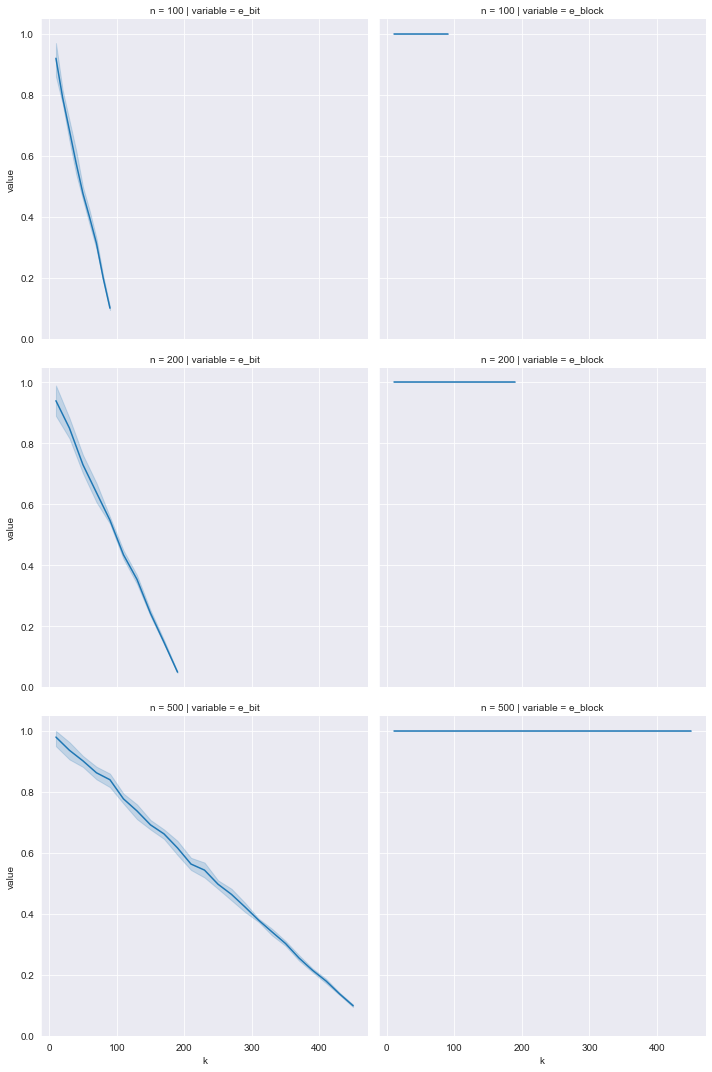
\includegraphics[width=0.6\textwidth]{figures/no-cleaning.png}
	  \end{figure}
        \item
	  \begin{figure}[H]
	    \centering
	    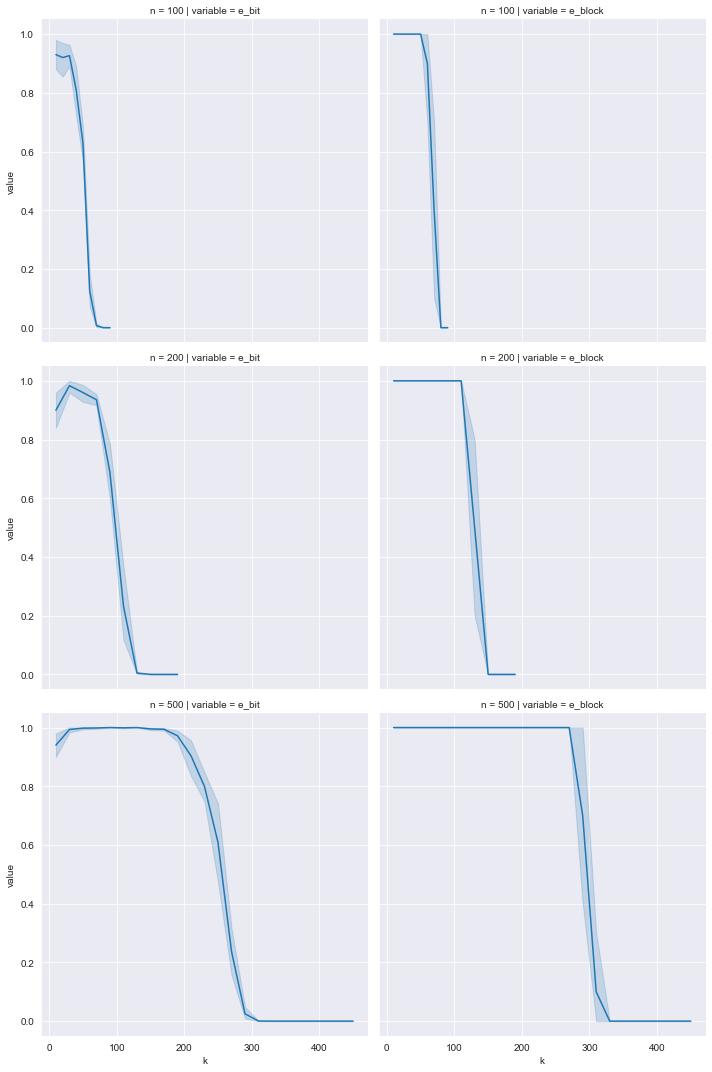
\includegraphics[width=0.6\textwidth]{figures/with-cleaning.png}
	  \end{figure}
	\item
	  TODO
    \end{enumerate}

\end{solution}

\end{document}
